\documentclass[12pt]{article}

% The geometry package allows for easy page formatting.
\usepackage[margin=20mm]{geometry}
\geometry{letterpaper}

% Load up special logo commands.
\usepackage{doc}

% Package for formatting URLs.
\usepackage{url}
\usepackage{hyperref}

\usepackage{braket}
\usepackage{bbold}
\usepackage{amsmath, amsfonts, amsthm}
\usepackage{amssymb}
\usepackage{pgfplots}
\usepackage{mathtools}

\usepackage{multicol}
\usepackage{wrapfig}
\usepackage{subfig}

% Packages and definitions for graphics files.
\usepackage{graphicx}
\graphicspath{ {./figures/} }		% path of images

\usepackage{epstopdf}
\DeclareGraphicsRule{.tif}{png}{.png}{`convert #1 `dirname #1`/`basename #1 .tif`.png}

%
% Set the title, author, and date.
%
\title{A Study on Star Clusters}
\author{Anthony Karoki Mugambi\\
	\small I44/1899/2018\\
	\small Department of Physics, University of Nairobi, Chiromo Campus, Nairobi, Kenya
}
\date{}

%
% Instantiate commands
%

\renewcommand{\thefootnote}{\fnsymbol{footnote}}  %use symbolic footnote

%
% Keywords command
\providecommand{\keywords}[1]
{
	\small	
	\textbf{\text{Keywords: }} #1
}


%
% The document proper.
%
\begin{document}
	\maketitle
	
	\begin{abstract}
		This paper presents a photometric study on star clusters. The focus is on both open and globular star clusters; specifically the open star cluster M7 and the globular star cluster M54. The photometric data for each cluster in study is collected from online databases that store data collected from various telescopes. The photometric data collected, majorly optical and infrared data, is the essential ingredient in the construction of the Colour-Magnitude Diagrams (CMD) of each star cluster. Plotting the CMD requires the visual magnitudes of each member star of the star clusters. Using theoretical isochrone models fitted onto the Colour-Magnitude Diagrams, approximate distances and ages of the star clusters are determined. Results on the distances and ages gained from this approximation method are compared to the actual distances and ages recognised, used and agreed upon by astrophysics studies.
		
	\end{abstract}

	\keywords{colour-magnitude diagrams, globular clusters, open clusters}
	
	%\pagebreak
	%\tableofcontents
	
	%\pagebreak
	%\listoffigures

	\pagebreak
	\section{Introduction}
	\label{sec:intro}
	Most stars in the universe form in clusters (Lada \& Lada 2003). Star clusters are groups of stars that share a common origin and are gravitationally bound together. The star clusters are formed at the same time and from the same gas cloud, and they thus have similar age and are found at a common relative distance as viewed from Earth. The common age and distance makes stellar clusters particularly important in studies and models of stellar evolution, stellar ages, metallicities and luminosities. For this reason, photometric measurements can be used to determine the age of a cluster and its distance as viewed from Earth.\\
	The two basic categories of stellar clusters are open clusters and globular clusters. Open clusters are diffuse star clusters hosting a few hundreds or thousands of stars. Individual component stars are easily resolved with telescopes hence the name open cluster. They are mostly found on the dusty spiral arms on the plane of spiral galaxies. In this paper, we shall look at the open cluster Messier 7 (M7) or NGC 6475.\\
	Globular clusters are spheroidal collections of several hundred thousands to a million stars found orbiting in the halos of all large galaxies. They tend to be very densely packed, hosting millions of stars in the space of only a few parsecs. They comprise the oldest stars in the galaxy. In this paper, we shall look at the globular cluster Messier 54 (M54) or NGC 6715.\\	
	The main motivation of behind the astrophysical study of stellar clusters is because they allow astronomers to improve on current the current model and knowledge bank of stellar evolution and ages of stars. By fact that this stars arose from the same molecular gas cloud, member stars in the cluster share effectively the same evolutionary trajectory.\\
	Also, the member stars are effectively at the same distance from an observer on Earth. We say this and more so why this is logically true is because the distance from the cluster to Earth is significantly greater than the distances among the stars spatially distributed within the cluster.\\
	Globular clusters appear to have formed shortly after the Big Bang, making them very old stellar systems, so they are used by astronomers to investigate how the universe was long ago. CMDs can be used to determine the properties of globular clusters, including their age and metallicity.\\
	On the other hand, open clusters, begin young stellar systems can teach us about stellar cluster formation and evolutionary properties and structures.\\
	For this project, CMD graphs for the two stellar clusters in study are constructed using infrared data. The colour of the many stellar cluster members are determined and plotted against their visual magnitude to generate a CMD. The CMD is just a type of Hertzsprung-Russell (HR) diagram in which plotting is done using the colour index (CI\footnote[1]{CI = B - V}) rather than spectral class (SC) on the horizontal axis; and the apparent visual magnitude, V, is used for the vertical axis. The apparent visual magnitude data is important in helping to infer the relative absolute magnitudes of stars in the cluster.\\
	Colour index is a simple numerical expression the determines the colour of an object. An object's luminosity is observed through two different filters, e.g. B and V (blue light and green-yellow visible light). The difference in the luminosities, i.e. B - V, is the colour index. A smaller colour index indicates a bluer hence hotter star while a larger colour index indicates a redder/cooler star.\\
	Apparent magnitude is a logarithmic measurement of the brightness of stars/celestial objects as viewed from Earth. It is based on how human eyes view different levels of brightness. It is denoted by \textbf{m} and measured in magnitudes.\\
	Absolute magnitude is a measurement of a star's/celestial object's brightness if it were located at a distance of 10 parsecs. It is a measure of the true brightness. It is denoted by \textbf{M} and measured in magnitudes. A star's magnitude tells us about its luminosity. On determining a star's absolute magnitude, one can estimate its distance from Earth. A star's colour also tells us about its surface temperature.\\
	The CMD plots are then overlaid with theoretical stellar evolution isochrone models to match and fit the turn-off points to be used to estimate the age of each target. Isochrones are adjustable models of data  sets. The turn-off point is the phase where stars leave off the main sequence. By applying isochrone fitting, measurements on the ages and distances of the open and globular clusters M7 and M54 respectively are made.\\
	The aim of this paper is to take on a study of the two types of star clusters to determine their age and distances and show show how, using photometric data, star clusters can be used to measure the relative distances and ages of stars in the cluster.
	
	
	
	%\pagebreak
	\section{Theory and Background Information}
		\subsection{Messier 7 Open Cluster}
		\begin{wrapfigure}{l}{0.6\textwidth}
			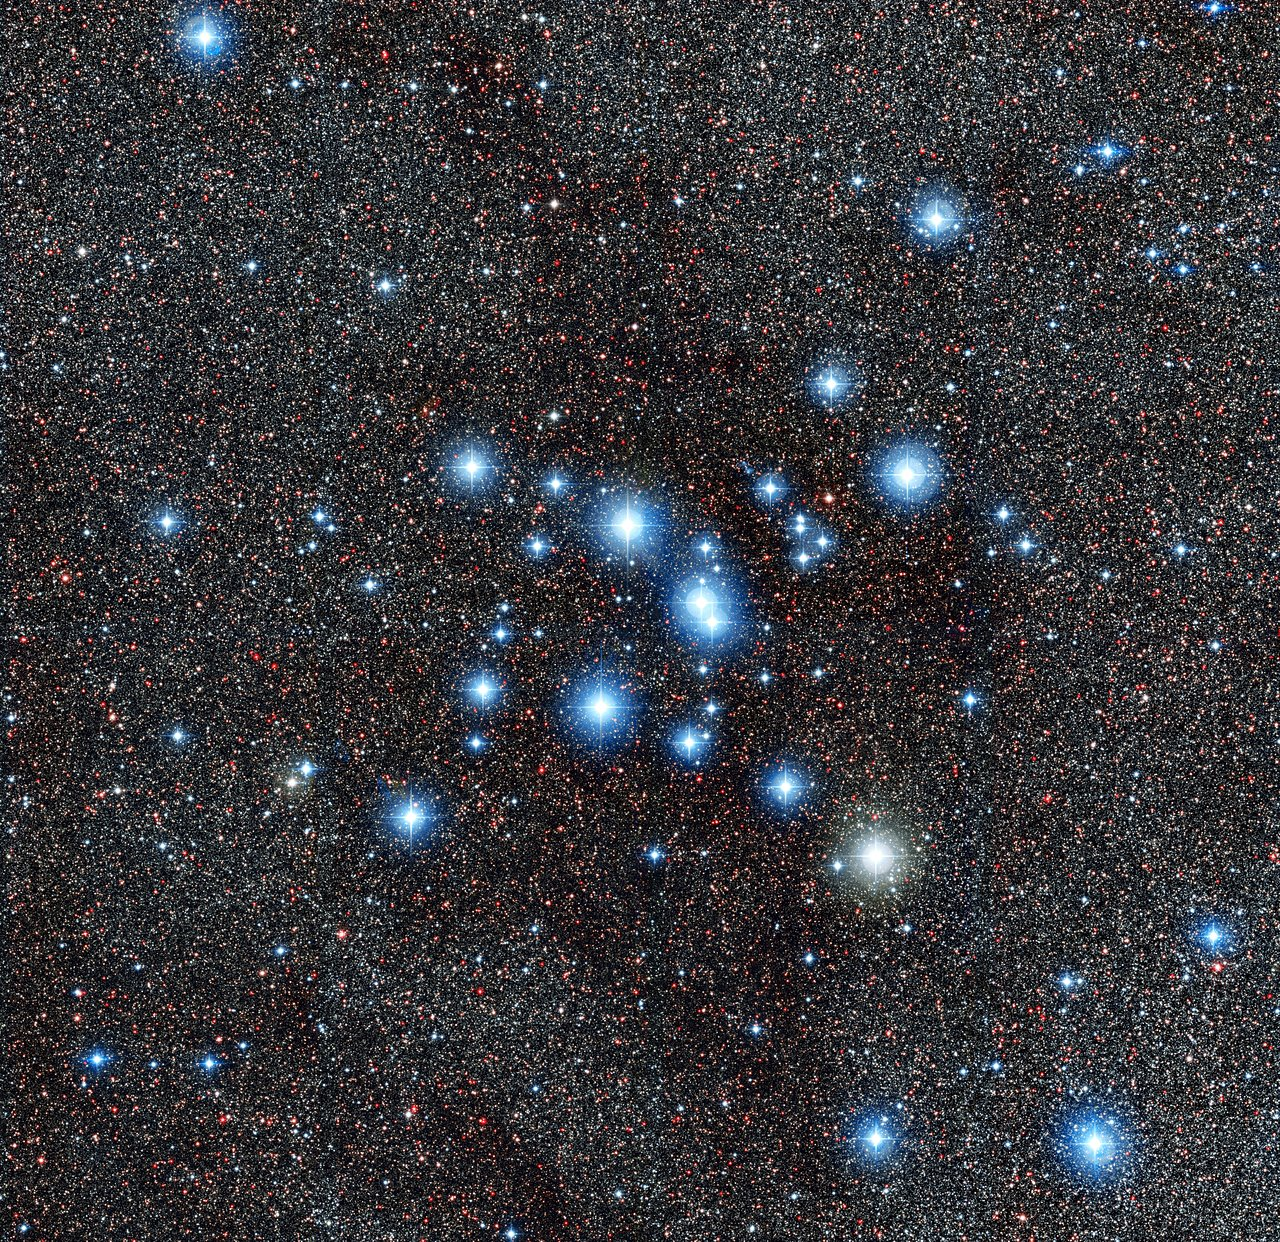
\includegraphics[width=0.58\textwidth]{m7_eso_0}
			\caption{This new image from the Wide Field Imager on the MPG/ESO 2.2-metre telescope at ESO’s La Silla Observatory in Chile, shows the bright star cluster Messier 7, also known as NGC 6475. Easily spotted by the naked eye in the direction of the tail of the constellation of Scorpius (The Scorpion), this cluster is one of the most prominent open clusters of stars in the sky and an important research target. (European Southern Observatory, ESO, 2014) \cite{eso_m7} Credit: ESO}
			\label{fig: m7}
		\end{wrapfigure}
		\textbf{M7} also goes by the designations \textbf{NGC 6475} and \textbf{Ptolemy's Cluster}. M7 was known as early as the year 130 CE when it was mentioned by Claudius Ptolemy, a 2$^{nd}$ century Greek Astronomer and Mathematician. It is a large prominent bright star cluster visible to the naked eye in the constellation Scorpius.\\
		It is part of the Milky Way galaxy. It has an apparent visual magnitude of 4.1 and its angular diameter is 80 arc-minutes making it easy to see with the naked eye. M7 lies at an estimated distance of 800 light years or about 300 parsecs. It's Right Ascension is 17h 53.9m while its Declination is -34° 49´ (AstroPixels, 2011) \cite{astropixels_m7}.\\
		Messier 7 contains about 80 stars between magnitudes 6 and 10. It is believed to be about 220 million years old and has a mass about 735 times that of the Sun. It is approaching us at a speed of 14 km/s. The brightest star in the cluster is a yellow G8-type giant with an apparent magnitude of 5.6.\\
		The stars in M7 were all formed at roughly the same time in the same large cosmic cloud and they therefore are an invaluable insight into stellar evolution and structure (Messier Objects, 2015) \cite{messier007}.\\
		\subsection{Messier 54 Globular Cluster}
		\textbf{M54} also goes by the designation \textbf{NGC 6715}. It is a compact globular cluster.\\
		It was the first extragalactic cluster ever discovered and is recognized as part of the Sagittarius Dwarf Galaxy (SDG), a satellite galaxy of the Milky Way (Hubble's Messier Catalog, 2017) \cite{nasa_m54}. It is located in the southern constellation Sagittarius. It has an apparent visual magnitude of 7.6 and its angular diameter is 9.1 arc-minutes. M54 lies at an estimated distance of 88,700 light years. It has a Right Ascension of 18h 55.1m and a Declination of -30° 29´.\\
		The estimated age of M54 is 13 billion years. Current estimates indicate that the M54 cluster, is situated almost 90 000 light-years away. Messier 54 occupies an area of 12 arc minutes, corresponding to a true radius of 153 light years.\\
		It is a quite concentrated and dense globular cluster with an absolute magnitude of -10 and a luminosity about 850,000 times that of the Sun (Messier Objects, 2015) \cite{messier54}.
		\begin{figure}%{l}{0.52\textwidth}
			\centering
			\subfloat[\centering Hubble image of M54 (ESA/Hubble) \cite{esahubble_images} Credit: ESA/Hubble $\&$ NASA]{{	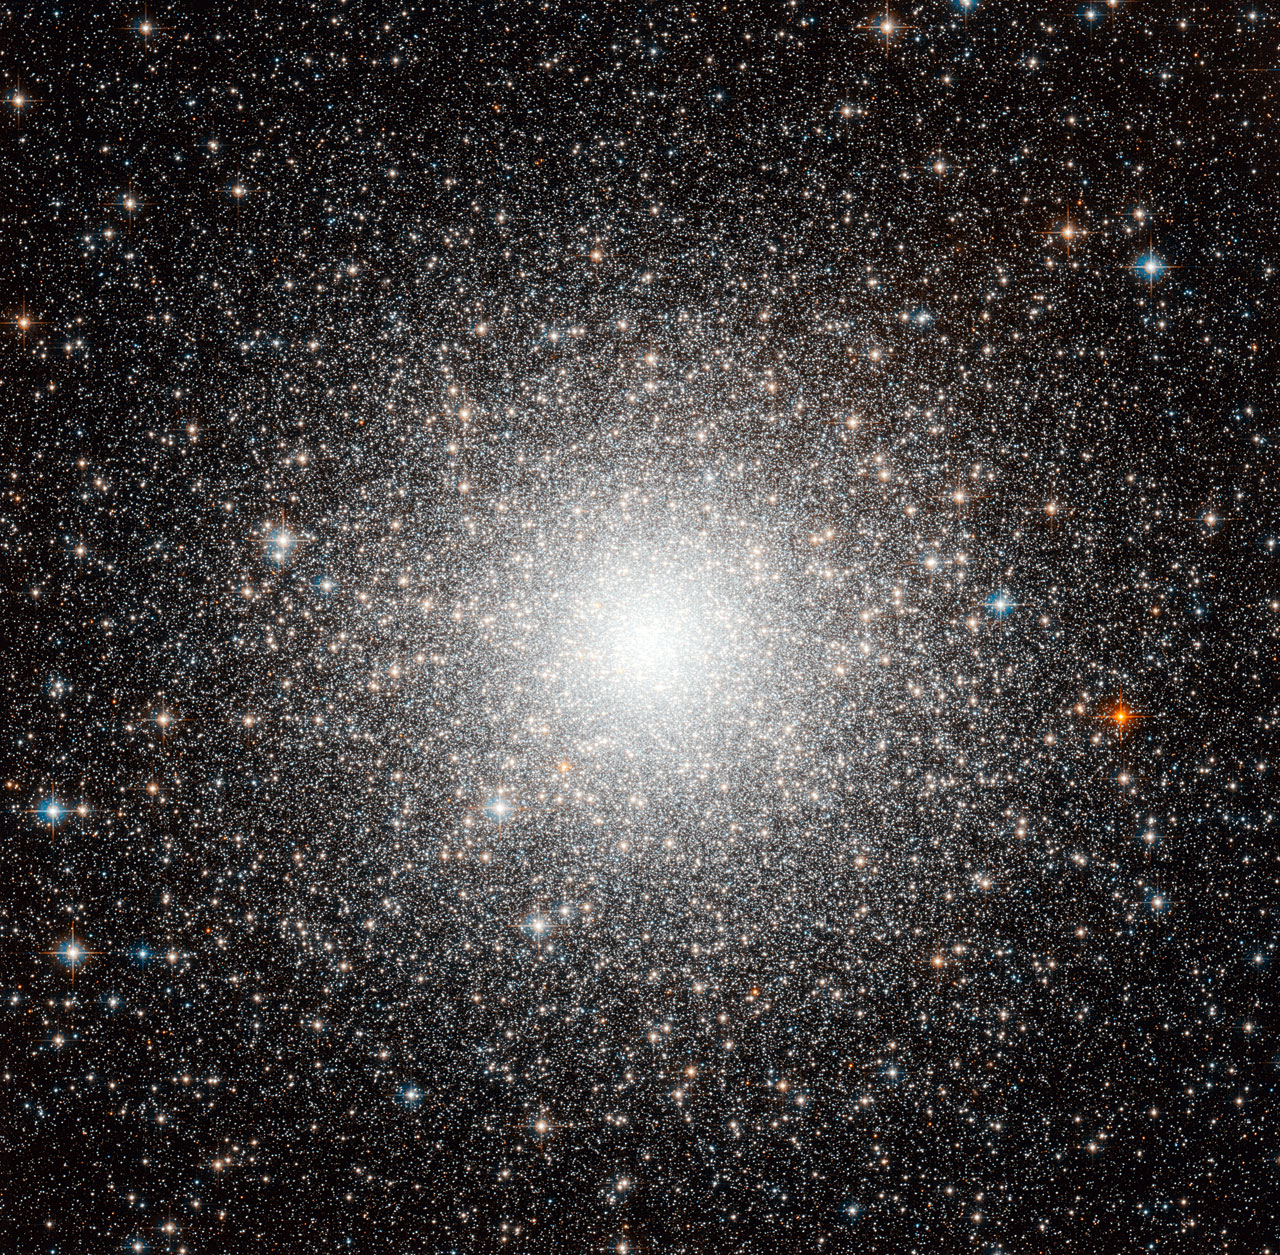
\includegraphics[width=0.5\textwidth, keepaspectratio]{m54_esa_nasa_hubble_0} }}
			%\qquad
			\subfloat[\centering This image from the VLT Survey Telescope at ESO’s Paranal Observatory in northern Chile shows the globular cluster Messier 54. This cluster looks very similar to many others, but it has a secret. Messier 54 doesn’t belong to the Milky Way, but actually is part of a small satellite galaxy, the Sagittarius Dwarf Galaxy. This unusual parentage has allowed astronomers to use the Very Large Telescope (VLT) to test whether unexpectedly low levels of the element lithium in stars are also found in  stars outside the Milky Way (European Southern Observatory, 2014) \cite{eso_m54} Credit: ESO]{{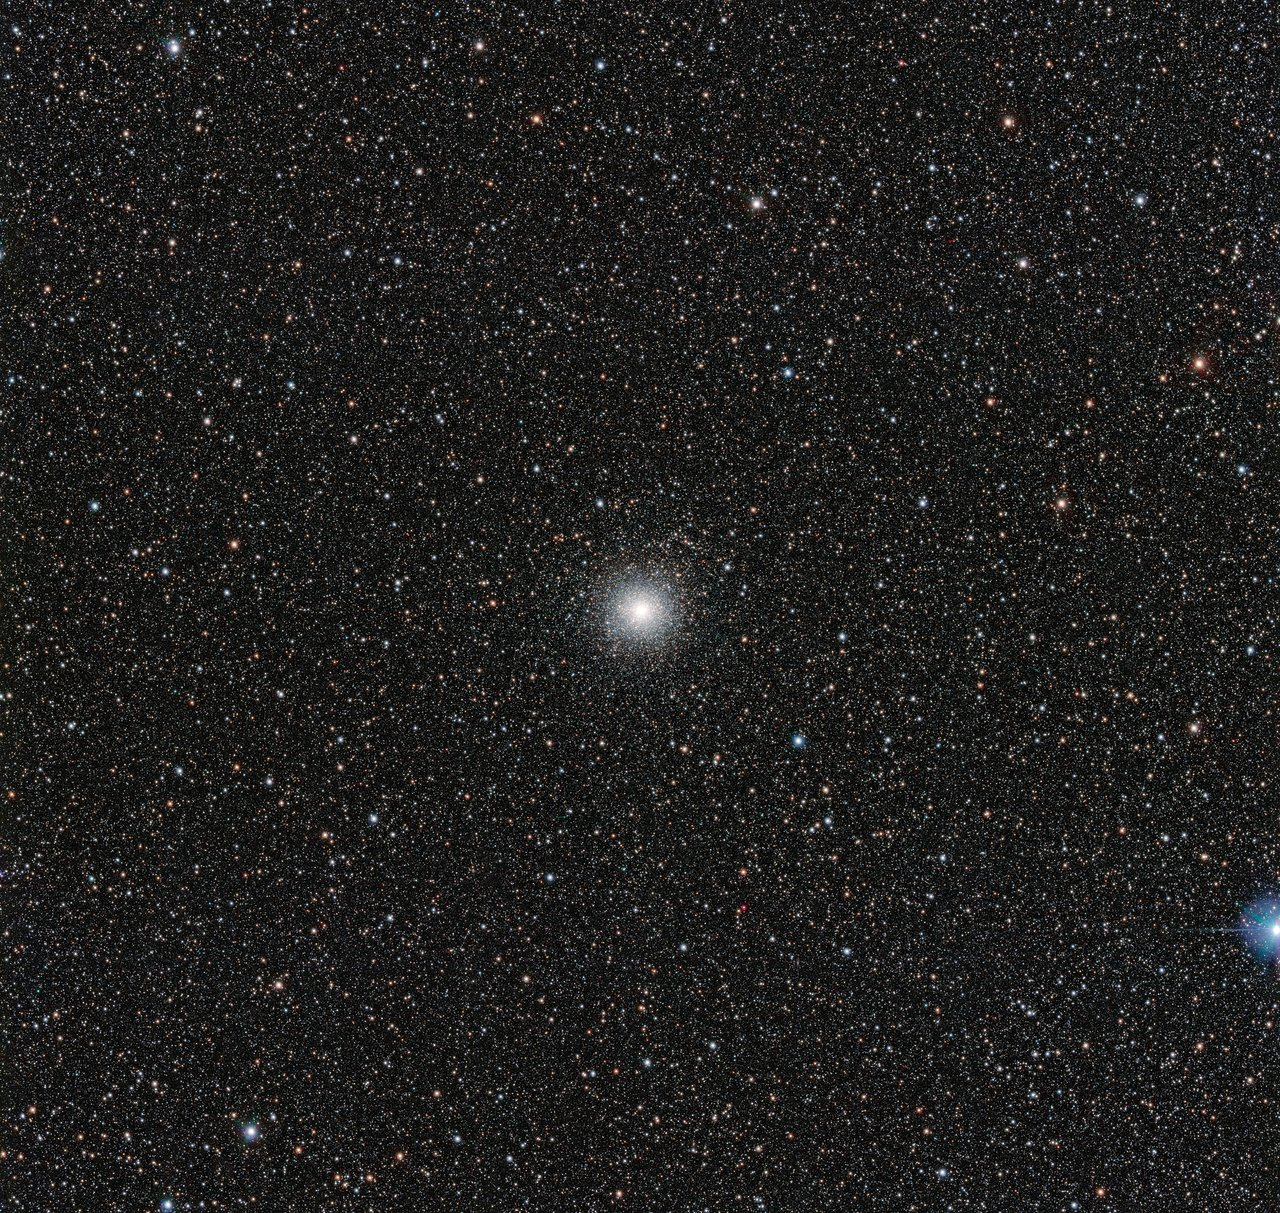
\includegraphics[width=0.5\textwidth, keepaspectratio]{m54_eso_0}}}
			\caption{M54 stellar cluster}
			\label{fig: m54_cluster}
		\end{figure}
%		\begin{figure}[h!]%{l}{0.5\textwidth}
%			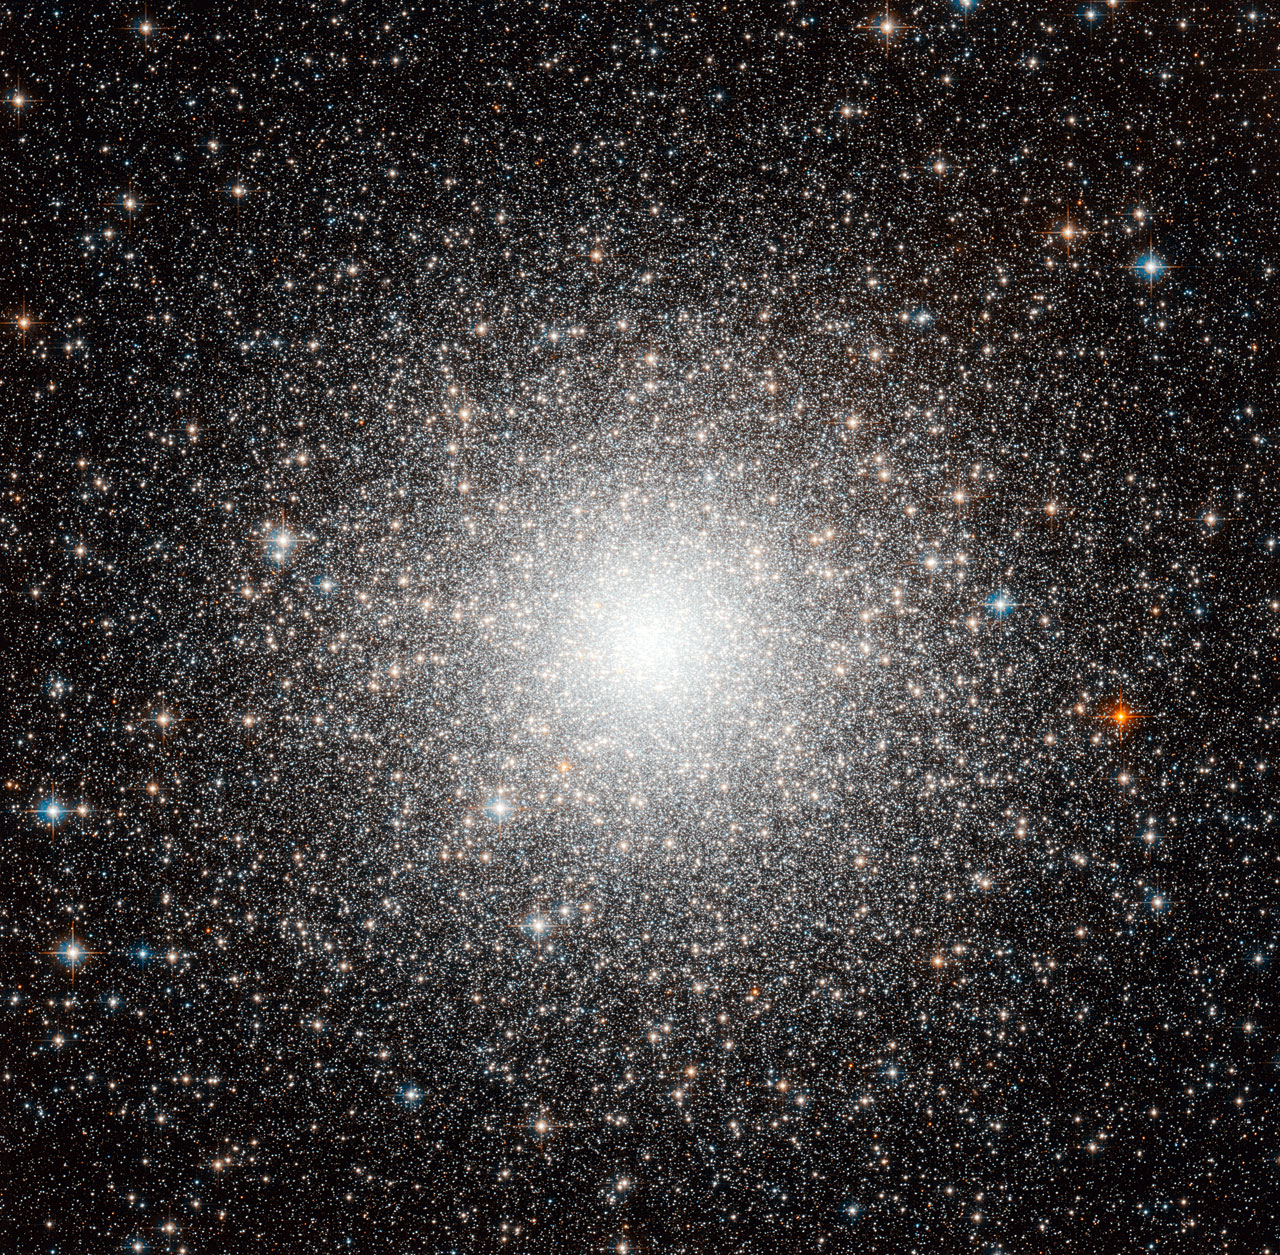
\includegraphics[width=0.5\textwidth]{m54_esa_nasa_hubble_0}
%			\caption{Hubble image of M54. \cite{esahubble_images}\\Credit: ESA/Hubble $\&$ NASA}
%			\label{fig: m54}
%		\end{figure}
%		\begin{figure}[h!]%{r}{0.5\textwidth}
%			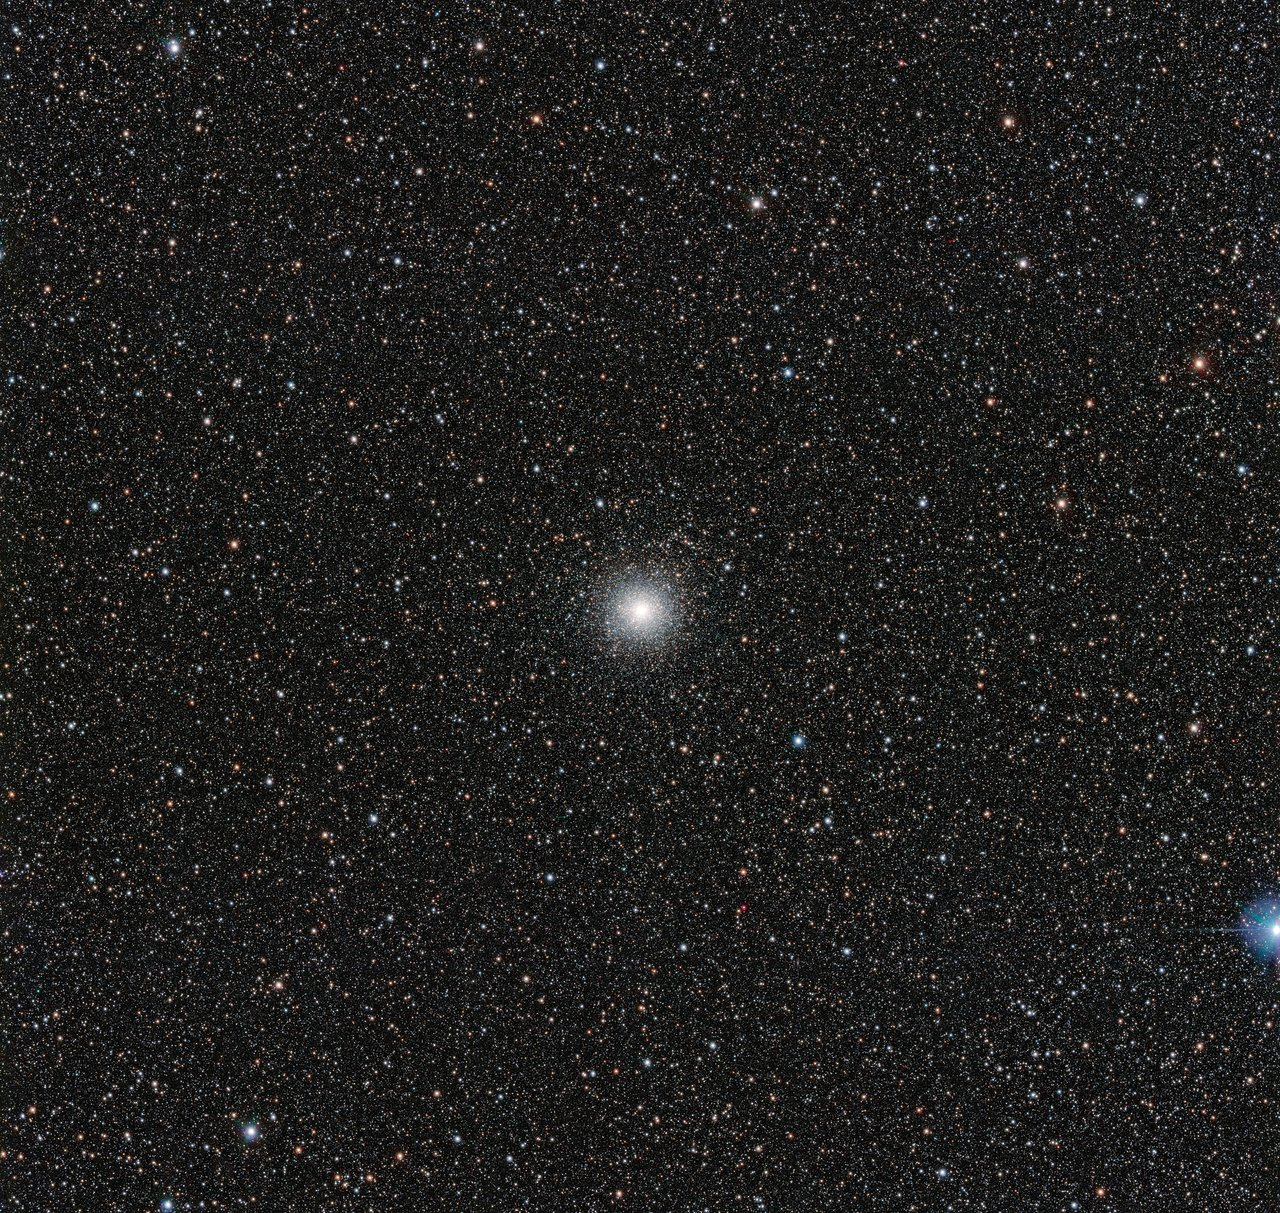
\includegraphics[width=0.5\textwidth]{m54_eso_0}
%			\caption{This image from the VLT Survey Telescope at ESO’s Paranal Observatory in northern Chile shows the globular cluster Messier 54. This cluster looks very similar to many others, but it has a secret. Messier 54 doesn’t belong to the Milky Way, but actually is part of a small satellite galaxy, the Sagittarius Dwarf Galaxy. This unusual parentage has allowed astronomers to use the Very Large Telescope (VLT) to test whether unexpectedly low levels of the element lithium in stars are also found in  stars outside the Milky Way. \cite{eso_m54}\\Credit: ESO}
%			\label{fig: m54_1}
%		\end{figure}	
	
	\pagebreak
	\section{Methodology and Procedure}
	Part of the methodology used to make photometric measurements to determine the age and distances of clusters is by taking photometric images of our clusters through separate colour filters. Since the images in use for this case are the 2MASS infrared images, we will make use of the J and K band filters, to measure the apparent magnitude of each star in each waveband colour. Our colour index (CI) is going to be given by\[CI = J - K\]
	The method being used in finding a star's brightness, among the many that exists, is the  aperture photometry method. This involves taking a whole image of a star cluster and narrowing in on each individual visible star and encircling it with an aperture that encircles all image pixels containing a part of the star's brightness. Algorithms in the APT tool perform computations of aperture photometry to determine each star's apparent magnitude.
		\subsection{Database}
		To get the data for the star clusters M7 and M54, the data archives from NASA/IPAC EXTRAGALACTIC DATABASE (NED) website are used. For each star cluster, the infrared data is found at the NASA/IPAC Infrared Science Archive page of the NED website. After getting the 2MASS Interactive Image Service Results, downloads of the J, K and H bands of the 2MASS Atlas images are made.
%		Aperture Photometry Tool (APT) is software with a graphical user interface for data and image visualization and computing aperture photometry on astronomical imagery. Image overlays, graphical representations, statistics, models, options and controls for aperture-photometry calculations are brought together into a single package.
		\subsection{Data Analysis}
		Having downloaded the J, H and K bands 2MASS images for each cluster, we move on to the data analysis procedures using the relevant software tools.\\
		The DS9 visualization tool can prove useful when comparing the J, H and K images to ensure they are the stars in each image band are well aligned and only the colour and luminosities are different.\\
		Normally, the methodology or procedure to follow is; plotting the visual magnitudes, V, of stars against their B-V colour indices. This will result in a graph that resembles a HR diagram.\\
		For this project's case however, the data in use is the infrared data. The three images downloaded are 3-band composites constructed from 2MASS Atlas images. The infrared images are then mapped into false colours so that they are visible to humans on the visible spectrum for easier visualization and human analysis. The 3 bands are named J, H and K.\\
		The J band is taken at a wavelength of $1.235\mu m$ and mapped into the false colour blue. The H band is taken at a wavelength of $1.662\mu m$ and mapped into the false colour green. The K band is taken at a wavelength of $2.159\mu m$ and is mapped into the false colour red.\\
		\subsubsection{Photometric Analsysis}
		The Aperture Photometry Tool (APT) is used to perform aperture photometry analysis on the images. For each cluster, we begin by opening a single image, say the J-band image to begin with. An essential setting to consider is the magnitude zero point. This is essential in calibrating the software to the standard magnitude system used by Atlas images. This parameter can be found in the image headers under the name MAGZP. For cluster M7, the magnitude zero point is $20.9474$ for the J-band and $19.8980$ for the K-band. For cluster M54, it is $20.8847$ for the J-band and $19.8916$ for the K-band.\\
		Also note that the pixel values for the Atlas images are in data-number (D.N) units.\\
		Next step is usually to recompute photometry of the image before creating a source list that contains data about all the stars in the cluster in that respective waveband. Finally, make an export of the data into a CSV file. The CSV file is a file with comma separated values. The same procedure should be followed for the K-band image as well.
		\subsubsection{Plots and Graphs}
		For this next procedure we make use of TOPCAT. Using TOPCAT, we open up the CSV data files that were exported from APT. The CSV file contains data in table form. The table columns of interest to us are the magnitude and magnitude uncertainty columns.\\
		We open up the CSV file containing data for the J-band, then open the CSV file containing data for the K-band. We proceed to match the two tables based on the exact value criteria/algorithm. This allows us to match table 1 to table 2 with the matched value column being the number parameter. The new combined data table will by default be called Match(1, 2).\\
		Display the Match(1, 2) table columns. Using the check boxes, we tick out the unnecessary data that we don't need. This is inclusive of every column except the columns on magnitude and magnitude uncertainty. We can rename those columns as; magnitude 1 renamed as J and magnitude uncertainty 1 renamed as err$\_$J while magnitude 2 renamed as K and magnitude uncertainty 2 renamed as err$\_$K.\\
		Next we create a new column for our colour index. Call this new column JK, assign it the expression $J - K$, with units of mag.\\
		We can now plot the data. We go to the plane plotting window provided by TOPCAT. We change the axes to our desired axes, that is, JK on the x-axis and J on the y-axis. We also flip the y-axis so that the smaller numbers are at the top because the brighter stars have smaller magnitudes.\\
		We now have our CMD plotting with the J magnitude against the JK colour index.
		
	\pagebreak
	\section{Results}
	We now have plots for our data. The plots actual data for the member stars in each star cluster. In the CMD plots, we see our Main Sequence and Red-Giant branches titled nearly vertically. Please see Figure ~\ref{fig: m7_cmd_apparent} for the M7 CMD plot and Figure ~\ref{fig: m54_cmd_apparent} for the M54 CMD plot.
		\begin{figure}[h!]
			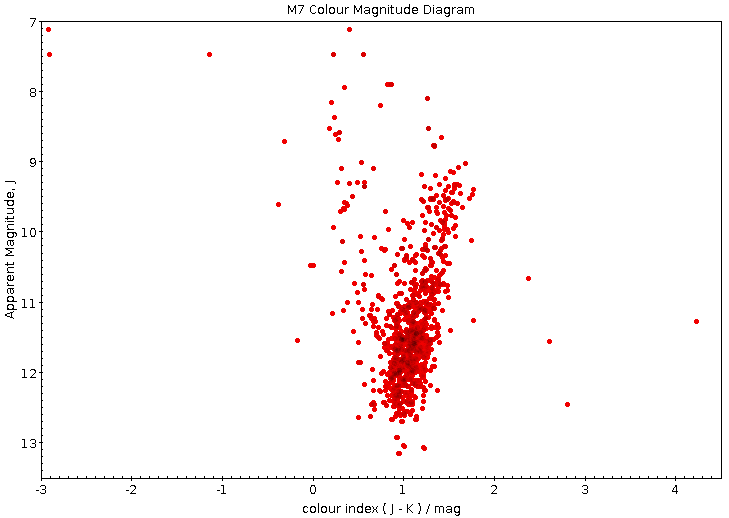
\includegraphics[width=\textwidth]{m7_cmd_apparent}
			\caption{M7 CMD plot using apparent magnitude}
			\label{fig: m7_cmd_apparent}
		\end{figure}
		\begin{figure}[h!]
			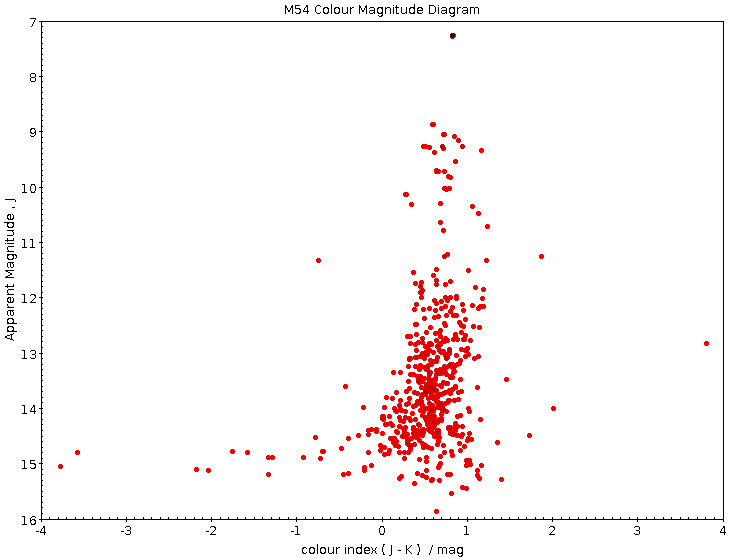
\includegraphics[width=\textwidth]{m54_cmd_apparent}
			\caption{M54 CMD plot using apparent magnitude}
			\label{fig: m54_cmd_apparent}
		\end{figure}
		\subsection{Applying for Corrections}
		The next step is accounting for the physical effects that affect the shape of the CMD diagrams. The biggest effect is the \textbf{galactic extinction}. Galactic extinction refers to the effect of dust and gases in the Milky Way galaxy that causes the apparent magnitudes to be greater than they are i.e. it dims the light of objects within the galaxy and beyond the galaxy (Zeilik and Gregory, 1998) \cite{zeilik}.\\
		Its effects are stronger at shorter wavelengths, resulting in starlight appearing redder than it normally is. This makes stars appear cooler. This shifts our J-K colour indices, hence our temperature estimates so that the stars are actually hotter than estimated (Danford \& Thomas 1981, Pandey et al., 2001) \cite{pandey}.\\
		We thus have to apply an extinction correction. We make use of the NASA/IPAC Extragalactic Database (NED). We go to their tab on galactic extinctions to get the correction magnitudes. We use the UKIRT J and UKIRT K bandpasses. For M7, the galactic extinction magnitudes are $0.512$ for UKIRT J and $0.218$ for UKIRT K. For M54, these are $0.108$ for UKIRT J and $0.046$ for UKIRT K.\\
		The mathematical expression for the corrected magnitudes is as follows:
		\[M_{J, corrected} = M_{J, observed} - M_{Galactic \,\, Extinction}\]
		We will adjust our model by the galactic extinction and re-plot the CMD plots. These corrected plots are seen in Figure ~\ref{fig: m7_m54_cmd_corrected}.
		\begin{figure}
			\centering
			\subfloat[\centering M7 corrected CMD plot using corrected apparent magnitude]{{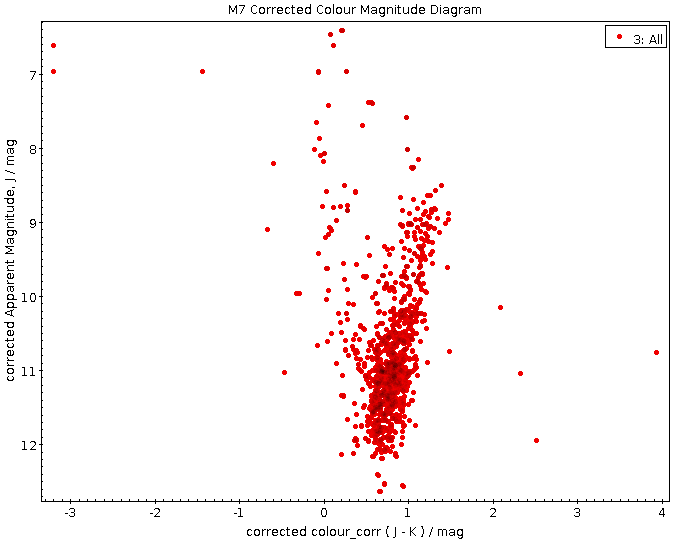
\includegraphics[width=0.7\textwidth, keepaspectratio]{m7_cmd_corrected_apparent}}}
			\qquad
			\subfloat[\centering M54 corrected CMD plot using corrected apparent magnitude]{{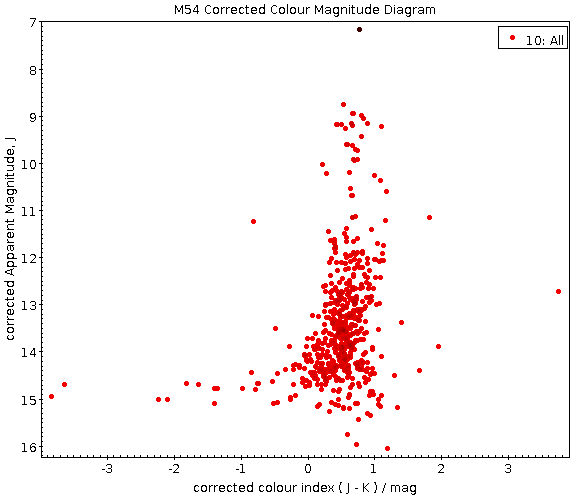
\includegraphics[width=0.7\textwidth, keepaspectratio]{m54_cmd_corrected_apparent}}}
			\caption{Extinction corrected CMD plots}
			\label{fig: m7_m54_cmd_corrected}
		\end{figure}
%		\begin{figure}
%			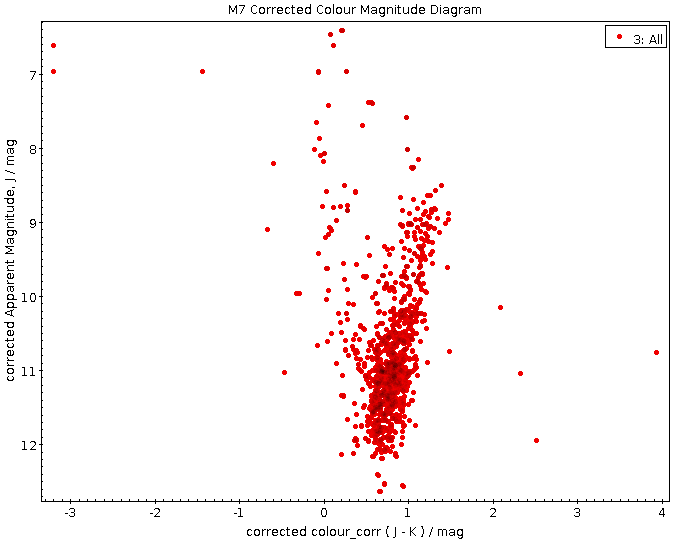
\includegraphics[width=\textwidth]{m7_cmd_corrected_apparent}
%			\caption{M7 corrected CMD plot using corrected apparent magnitude}
%			\label{fig: m7_cmd_corrected}
%		\end{figure}
%		\begin{figure}
%			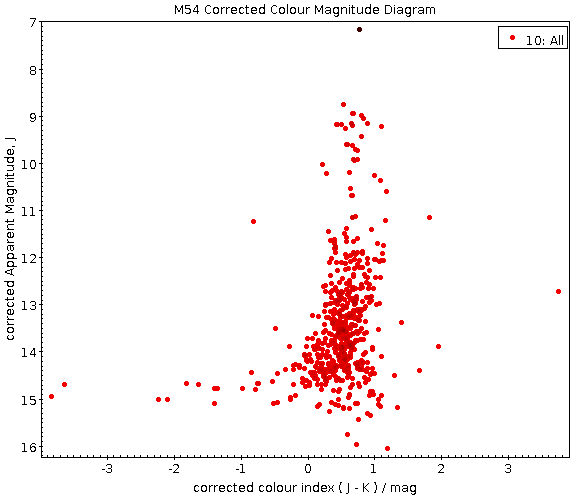
\includegraphics[width=\textwidth]{m54_cmd_corrected_apparent}
%			\caption{M54 corrected CMD plot using corrected apparent magnitude}
%			\label{fig: m54_cmd_corrected}
%		\end{figure}

		\pagebreak
		\subsection{Finding Age and Distance}
		The approach into solving this process involves overlaying and fitting a theoretical stellar model isochrone. The best fitting isochrone to the CMD gives the best approximate measurement of age and distance. It is a fact that the absolute magnitudes of stars in different star clusters have some differences. However, using this method, we can fit a theoretical model of a cluster's stars to its Colour Magnitude Diagram. In this isochrone computer model, all stars have the same age, just as we would expect for clusters. In practice, the isochrone is a table os simulated stars, one star per row where the star columns give the star's absolute magnitude in different filters.\\
		The resource website for getting the isochrone models is called CMD 3.4 input form and it is found at \url{http://stev.oapd.inaf.it/cgi-bin/cmd}. It is a web interface dealing with stellar isochrones and their derivatives. We can download isochrones of different ages until and plot a for for each one till we get a satisfactory fit that is closest to our CMD plot.\\
		We choose our photometric system as 2MASS JHKs. Next important section is the Ages/metallicities input information section. We will enter the desired age in initial value input box. Globular clusters tend to be old, thus we will use ages ranging from 1-14 Billion years (Bradely and Dale, 2014) \cite{bradley}. Since open clusters tend to be younger, our age ranges can be from 50-900 Million years (Bradely and Dale, 2014) \cite{bradley}.\\
		We choose 200e6 or 200 Million years for our M7 open cluster and 13e9 or 13 Billion years for our M54 globular cluster.\\
		Submit the input data and download the ASCII isochrone files.\\
		Load and open them up in TOPCAT. Open up their column metadata and de-select every column except the magnitude columns; in this case it is labelled Jmag and Ksmag. Note that the magnitude values for the J and K bands are absolute magnitudes, while our CMD uses apparent magnitudes.
		\subsubsection{Cluster Distance}
		When we overlay the two plots, i.e. the CMD and the isochrone plot, we observe a clear average difference in the plots. The isochrone models plots are vertically above the CMD plots. This is due to the difference in the absolute and apparent magnitudes. The vertical axis of the CMD is representative of apparent visual magnitude while that of the isochrones is representative of absolute visual magnitude.\\
		This difference is called \textbf{distance modulus}. The distance modulus is given by
		\[\text{distance modulus}, \,\,\,\, \left(m - M\right) = 5\log_{10}(d) - 5\]
		\[\text{where}; \,\, m = \text{apparent magnitude}, \]
		\[ \,\,\,\,\,\,\,\,\,\,\,\,\,\,\,\,\, M = \text{absolute magnitude}, \]
		\[ \,\,\,\,\,\,\,\,\,\,\,\,\,\,\,\,\, d = \text{distance in parsecs}\]
		The distance modulus from the best fitting isochrone provides the best approximate distance and age measurements. Therefore, we can get our distance as
		\begin{equation}
			d = 10^{\frac{m - M + 5}{5}}
		\end{equation}
		The CMD plots overlayed with the isochrones can be seen in Figure ~\ref{fig: m7_m54_distance_modulus}.\\
		\begin{figure}
			\centering
			\subfloat[\centering M7 corrected CMD plot using corrected apparent magnitude overlayed against isochrone]{{	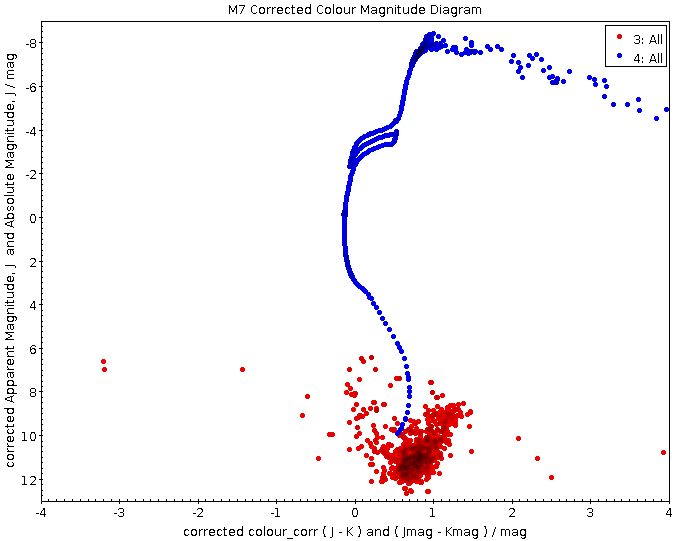
\includegraphics[width=0.7\textwidth, keepaspectratio]{m7_cmd_distance_modulus}}}
			\qquad
			\subfloat[\centering M54 corrected CMD plot using corrected apparent magnitude overlayed against isochrone]{{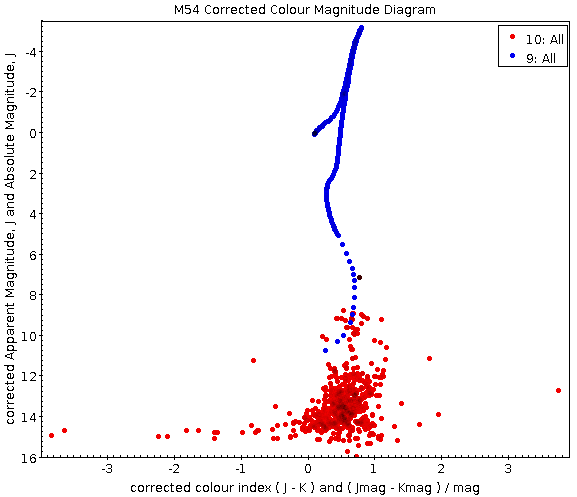
\includegraphics[width=0.7\textwidth, keepaspectratio]{m54_cmd_distance_modulus}}}
			\caption{Extinction corrected CMD plots overlayed against isochrone plots}
			\label{fig: m7_m54_distance_modulus}
		\end{figure}
%		\begin{figure}
%			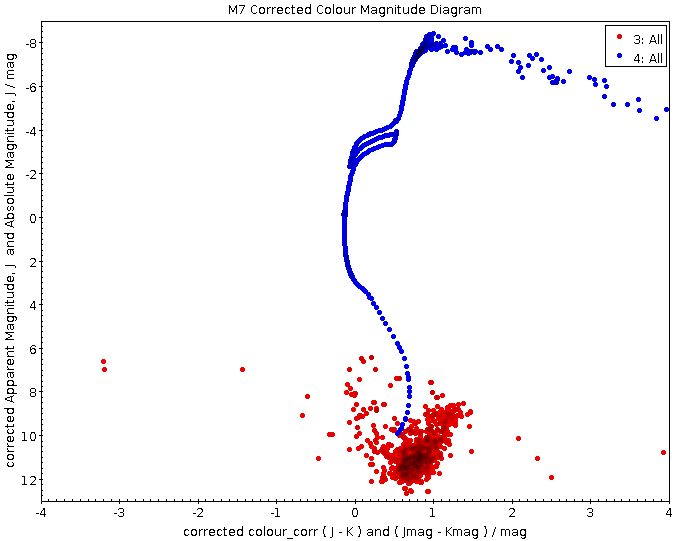
\includegraphics[width=0.5\textwidth, keepaspectratio]{m7_cmd_distance_modulus}
%			\caption{M7 corrected CMD plot using corrected apparent magnitude overlayed against isochrone}
%			\label{fig: m7_cmd_distance_modulus}
%		\end{figure}
%		\begin{figure}
%			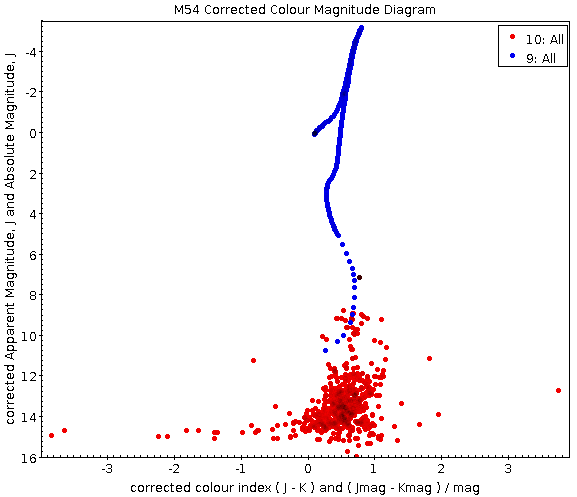
\includegraphics[width=0.5\textwidth, keepaspectratio]{m54_cmd_distance_modulus}
%			\caption{M54 corrected CMD plot using corrected apparent magnitude overlayed against isochrone}
%			\label{fig: m54_cmd_distance_modulus}
%		\end{figure}
		\\
		In order to scale down the isochrone plot, we identify, from the overlayed plotting, the distance modulus i.e. the magnitude difference between the plots, and add it to the absolute magnitude value of the isochrone. This will give us the apparent magnitude of the isochrone.\[M_{isochrone} + (m_{isochrone} - M_{isochrone}) = m_{isochrone}\]
		Plotting the isochrone using the apparent magnitude aligns it with the rest of the CMD plot.\\
		For the open cluster M7, we find the distance modulus to be about $7.5$. We can now use the distance formula as
		\[d = 10^{\frac{7.5 + 5}{5}} = \framebox{316.23 parsecs}\]
		This gives us an approximate distance to M7 as 316 parsecs.\\
		For the globular cluster M8, we find the distance modulus to be about $16.9$. Using the distance formula
		\[d = 10^{\frac{16.9 + 5}{5}} = \framebox{23, 988.33 parsecs}\]
		The globular cluster M54 is approximately at a distance of 24Kpc.
		\begin{figure}
			\centering
			\subfloat[\centering M7 corrected CMD plot using corrected apparent magnitude overlayed against isochrone]{{	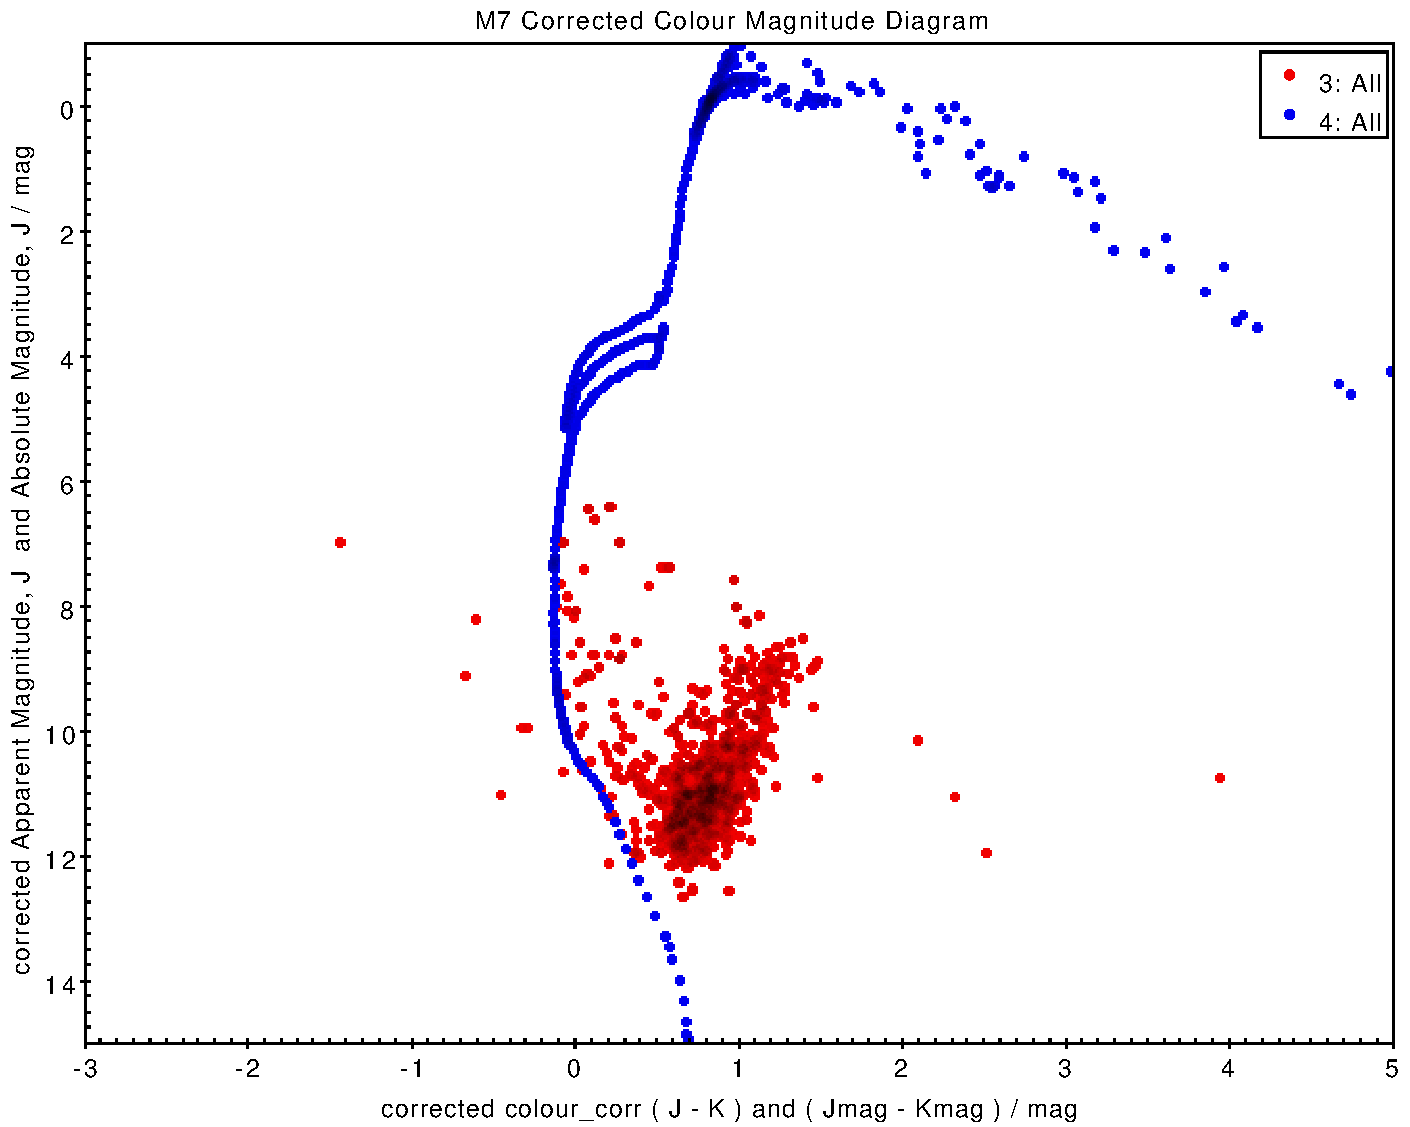
\includegraphics[width=0.7\textwidth, keepaspectratio]{m7_cmd_all}}}
			\qquad
			\subfloat[\centering M54 corrected CMD plot using corrected apparent magnitude overlayed against isochrone]{{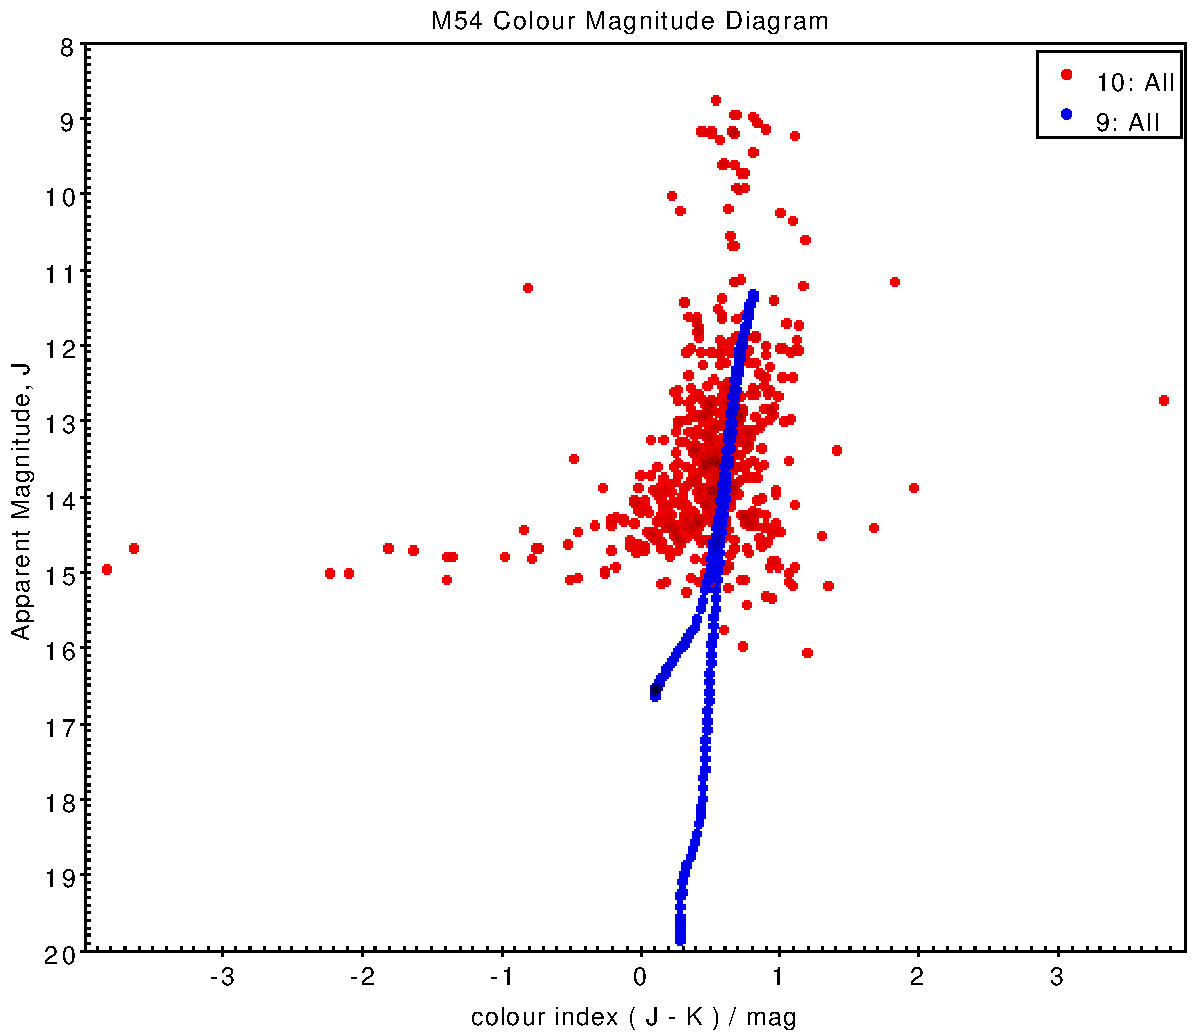
\includegraphics[width=0.7\textwidth, keepaspectratio]{m54_cmd_all}}}
			\caption{Extinction corrected CMD plots overlayed against isochrone plots with no distance modulus. Without distance modulus, the isochrone curves now use apparent magnitude and can fit in with the CMD plot.}
			\label{fig: m7_m54_all}
		\end{figure}
%		\begin{figure}
%			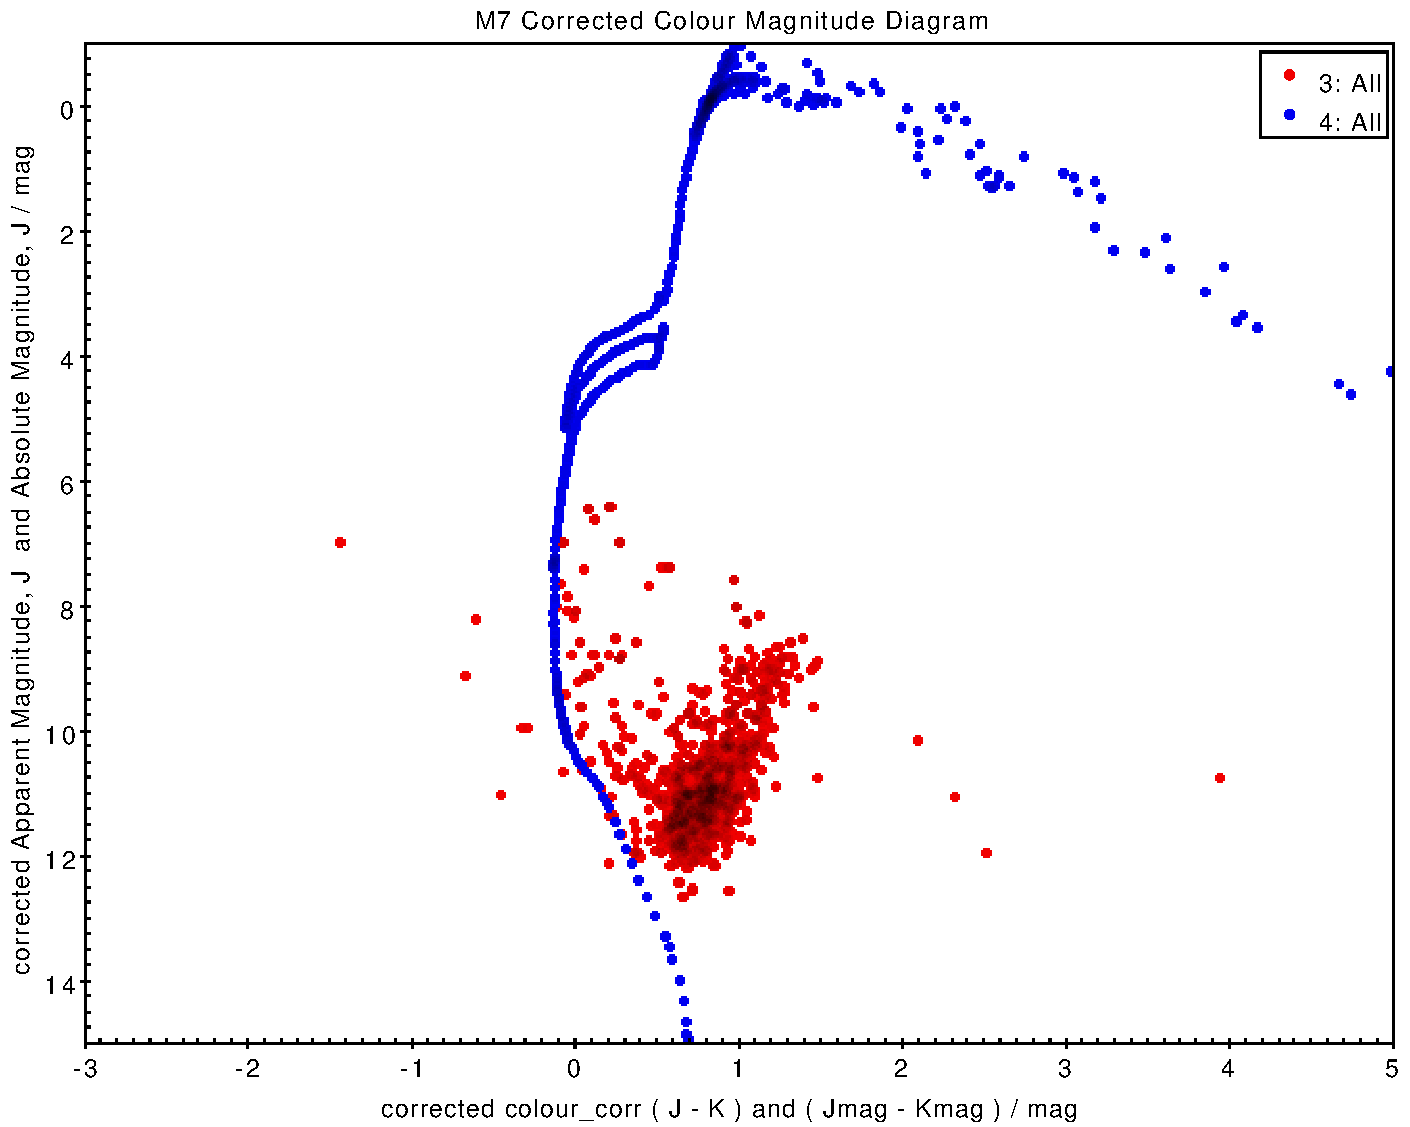
\includegraphics[scale=0.34]{m7_cmd_all}
%			\caption{M7 corrected CMD plot using corrected apparent magnitude overlayed against isochrone}
%			\label{fig: m7_cmd_all}
%		\end{figure}
%		\begin{figure}
%			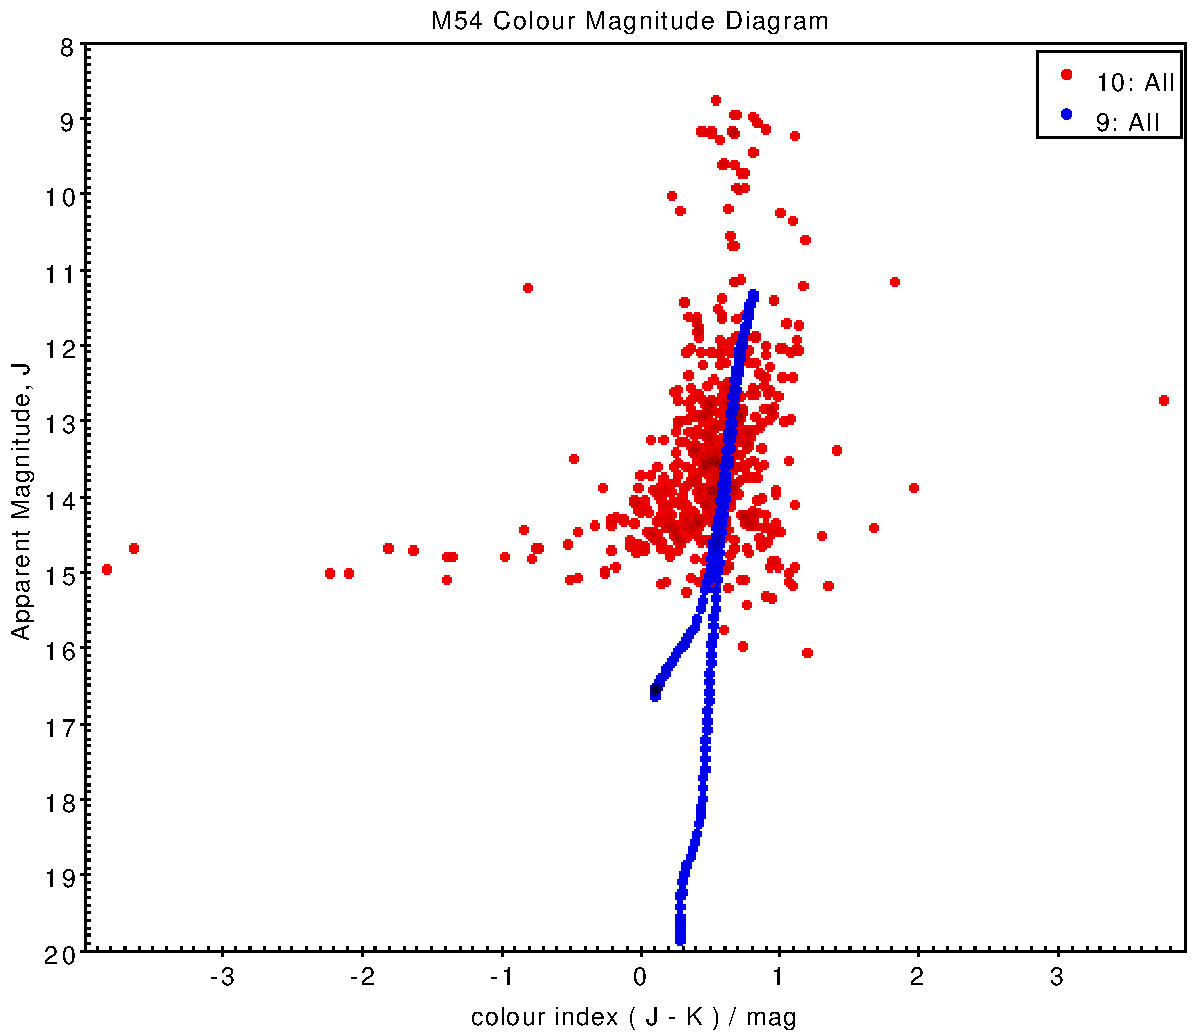
\includegraphics[scale=0.34]{m54_cmd_all}
%			\caption{M54 corrected CMD plot using corrected apparent magnitude overlayed against isochrone}
%			\label{fig: m54_cmd_all}
%		\end{figure}
		\pagebreak
		\subsubsection{Cluster Age}
		The age of a cluster is usually determined by the life expectancy of the most massive main sequence. We call this the \textbf{turnoff point}. Massive stars burn through their nuclear fuel much faster than their smaller main sequence counterparts.
		\begin{figure}[h!]%{l}{0.60\textwidth}
			\centering
			%\vspace{-30mm}
			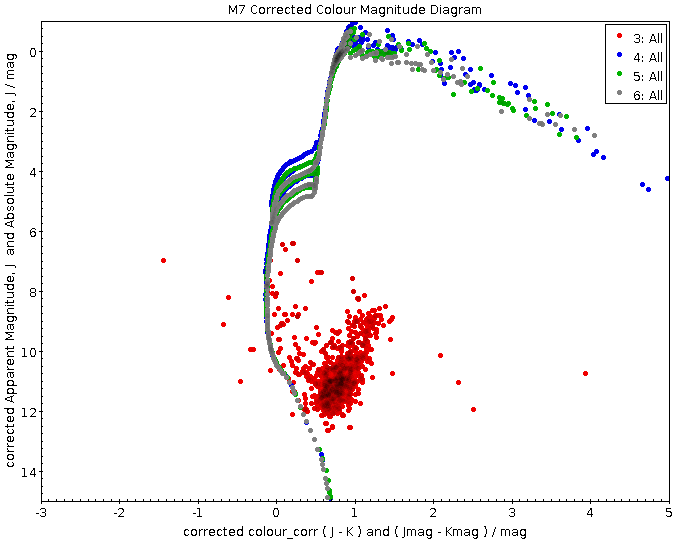
\includegraphics[width=0.95\textwidth, keepaspectratio]{m7_cmd_all_fits}
			\caption{3 isochrone overlays on M7 CMD plot}
			\label{fig: m7_cmd_all_fits}
		\end{figure}
		It should come as no surprise then that the most massive star main sequence star in the cluster will be the first one to evolve off from the main sequence (Albrecht and Bodo, 2001) \cite{albrecht}. Such a star also happens to be the most luminous of all main sequence star in the cluster.\\
		Normally on a HR diagram or CMD plot, this turnoff point appears as a bend in the otherwise linear shape of the main sequence.\\
		Overlaying the theoretical stellar evolution isochrones helps us determine the age of the cluster. The best choice fit isochrone for our CMD places both age and metallicity constraints on the stellar population. Using the downloaded isochrone data tables, we overlay as many as possible on our CMD to get a suitable fit as can be seen in the CMD plot for M7 in Figure ~\ref{fig: m7_cmd_all_fits}. The best for isochrone for the open cluster M7 had an age constraint of 200 Million years while for the M54 globular cluster, the age constraint was 13 Billion years.
		
	
	\section{Discussion}
	The colour of a star is usually determined by its surface temperature. Cooler stars are redder while mode blue stars are hotter. Stars in open clusters are typically young and their star's relatively small making them quite hot on the surface. Thus, on a HR or CMD diagram, many of these stars will appear on the blue parts of the spectrum.\\
	Since stars in globular clusters tend to be older and very large, they tend to have a cooler surface. On a HR or CMD diagram, they will mostly reside on the redder parts of the spectrum.\\
	From the plots, one can see that the stars on the open cluster M7 have lower colour indices and are therefore more blue in colour.\\
	For the globular cluster M54, the stars cover a much larger range of colour indices but are mostly in the larger values of the colour indices.\\
	The plots also had a few scattered points, but because of their scarce number, they are most likely just possible outgrowers.\\
	Of notice when it came to correction, only galactic extinction was taken into account. Reddening correction and atmospheric correction was not performed on the data, which would end up affecting the measurements, hence results.
		\subsection{Comparison with Archive Data}
		We compare results we got with from the CMD analysis with that obtained by various researchers and published in archive databases. We compare with data obtained from WEBDA and NED.
		\subsubsection{M7 Data Comparison}
		It is found that distance to M7 is 316.23 parsecs from our measurements. From WEBDA, the distance given is 301 parsecs. This is a very near accurate estimate, only off by about $5\%$.\\
		The age of M7 we found to be 200 Million years which is in close agreement to that given in the WEBDA database which is 220 Million years, making out measurements off by about $9\%$.
		\subsubsection{M54 Data Comparison}
		The established distance to M54 we found to be $23,988.33$ parsecs. The NED website data gives an estimated distance of $26,800$ parsecs or $87,400$ light years. This makes our distance measurements at about $10.5\%$ off of the actual distance.\\
		The best isochrone fit for the M54 CMD had an age of 13 Billion years; pretty much in accoradance with the NED website.
	\section{Conclusion}
	This work served as a proof of concept on how stellar cluster ages and distances can be determined from their luminosity. We observed photometric measurements of ages and distances of two star clusters, the open cluster M7 and the globular cluster M54, based on stellar evolution calculations and isochrone fitting models.\\
	The method of age and distance works satisfactorily. If we included metallicity, reddening offsets and corrected for earth's atmosphere, the calculations would be more accurate.\\
	Our overall conclusion is that studying star clusters using Colour Magnitude Diagrams and with appropriate theoretical methods of isochrone fitting can provide valuable new insights into stellar clusters as well as satisfactorily determine stellar distances and ages.
		
	\pagebreak
	\begin{thebibliography}{}
		
		\bibitem{albrecht}
		{Albrecht Uns\"{o}ld and Bodo Baschek},
		{The New Cosmos: An Introduction to Astronomy and Astrophysics},
		{Springer},{fifth edition}, 2001.
		
		\bibitem{bradley}
		{Bradely W. Carrol and Dale A. Ostlie},
		{An Introduction to Modern Astrophysics}
		{Pearson Education Limited},
		{second edition}, 2014.
		
		\bibitem{zeilik}
		{Michael Zeilik and Stephen A. Gregory},
		{Introductory Astronomy and Astrophysics},
		{Thomson Learning}, 1998.
		
		\bibitem{nasa_m54}
		{Hubble's Messier Catalog: Messier 54},
		{\url{https://www.nasa.gov/feature/goddard/2017/messier-54}},
		{[Last updated; Oct 19, 2017]},
		{[Online; accessed April 19, 2021]}
		
		\bibitem{messier54}
		{Messier Objects: Messier 54},
		{\url{https://www.messier-objects.com/messier-54/}},
		{[Last updated; June 10, 2015]},
		{[Online; accessed April 26, 2021]}
		
		\bibitem{messier007}
		{Messier 7: Ptolemy's Cluster},
		{\url{https://www.messier-objects.com/messier-7-ptolemys-cluster/}},
		{[Last updated; February 11, 2015]},
		{[Online; accessed April 16, 2021]}
		
		\bibitem{astropixels_m7}
		{M7 - Ptolemy Cluster},
		{\url{http://astropixels.com/openclusters/M7-01.html}},
		{[Last updated; 2011 June 28]},
		{[Online; accessed April 19, 2021]}
		
		\bibitem{esahubble_images}
		{Image Archive: Star Clusters},
		{\url{https://esahubble.org/images/archive/category/starclusters/}},
		{[Online; accessed April 19, 2021]}
		
		\bibitem{eso_m7}
		{The star cluster Messier 7},
		{\url{https://www.eso.org/public/images/eso1406a/}},
		{[Online; accessed April 19, 2021]}
		{[Release date: 19 February 2014, 12:00]}
		
		\bibitem{eso_m54}
		{The globular star cluster Messier 54},
		{\url{https://www.eso.org/public/images/eso1428a/}},
		{[Online: accessed April 19, 2021]}
		{[Release date: 10 September 2014, 12:00]}
		
		\bibitem{lada}
		{Lada C. J., Lada E. A.},
		{2003},
		{ARA\&A, 41, 57}
		
		\bibitem{pandey}
		{Pandey, A. \& Nilakshi, \& Ogura, K. \& Sagar, Ram \& Tarusawa, K.. (2001). NGC 7654: An interesting cluster to study star formation history. Astronomy \& Astrophysics - ASTRON ASTROPHYS. 374. 504-522. 10.1051/0004-6361:20010642.}
		
	\end{thebibliography}


\end{document}